\documentclass[a4paper, 11 pt]{article}


\usepackage{amsfonts}
\usepackage{amsmath}
\usepackage{amsthm}
\usepackage{appendix}
\usepackage{bm}
\usepackage{booktabs}
\usepackage[usenames, dvipsnames]{color} 
\usepackage{graphicx}
\usepackage{epstopdf}
\epstopdfsetup{update}
\usepackage{helvet}
\usepackage{hyperref}
\usepackage{indentfirst}
\usepackage{lscape}
\usepackage{morefloats}
\usepackage{natbib} \bibliographystyle{abbrvnat}\bibpunct{(}{)}{;}{a}{,}{,}
\usepackage{setspace}
\usepackage{subcaption}
\usepackage[capposition=top]{floatrow}
\usepackage{subfloat}
\usepackage[latin1]{inputenc}
\usepackage{tikz}
\usetikzlibrary{trees}
\usetikzlibrary{decorations.markings}


\theoremstyle{plain}
\newtheorem{thm}{Theorem}
\newtheorem{cor}{Corollary}
\newtheorem{lem}[thm]{Lemma}
\newtheorem{proposition}{Proposition}
\newtheorem{assumption}{Assumption}
\newtheorem{definition}{Definition}

%MARGINS
 \topmargin   =  7.0in
 \headheight  =  2.0in
 \headsep     =  0.7in
 \oddsidemargin= 0.0in
 \evensidemargin=0.0in
 \textwidth   =  6.45in
 \headheight  =  0.0in
 \topmargin   =  0.0in
 \textheight  =  9.0in
 \textwidth   =  6.45in
\setlength{\parindent}{4em}
\setlength{\parskip}{1em}

\newcommand{\fmt}{.eps}
%\newcommand{\fmt}{.png}
\hypersetup{                                                                                                    
    colorlinks=true,   
    linkcolor=BlueViolet,
    citecolor=BlueViolet,
    filecolor=BlueViolet,
    urlcolor=BlueViolet
}  




\setcounter{page}{0}
\begin{document}



\title{Fertility Timing and Season of Birth:\\ The Role of Biological and Economic Constraints\thanks{\scriptsize{We thank ... for helpful comments and suggestions. ... Any errors contained in the paper are our own.}}}
\author{Damian Clarke \\ U. of Oxford \and Sonia Oreffice \\ U. of Surrey \& IZA  \and Climent Quintana-Domeque \\ U. of Oxford \& IZA}
\date{April 2015}


%\author{Damian Clarke  \and Sonia Oreffice  \and Climent Quintana-Domeque  }
%\author{Damian Clarke \\ University of Oxford \and Sonia Oreffice \\ University of Surrey and IZA \and Climent Quintana-Domeque \\University of Oxford and IZA}


\maketitle
\thispagestyle{empty}

\begin{abstract}
{....}
\end{abstract}
\emph{JEL Classification Codes}: ....\\
\emph{Keywords}: .....


\newpage
\begin{spacing}{1.2}

\section{Introduction}
\section{Conceptual Framework}
\subsection{Two types of models}
\begin{itemize}
  \item First part of the paper: Modeling Season of Birth: biological constraints
  \item Second part of the paper: Modeling Fertility Postponement: biological + economic constraints. Why two types of mothers?
\end{itemize}

\subsection{Understanding Season of Birth Patterns: A Toy Model}
Suppose there are two seasons of birth, $T=\{0,1\}$: $\mathbf{0}$ ($Q4(t-1)\;,\;Q1(t)$) and $\mathbf{1}$ ($Q2(t)\;,\;Q(3)t$).

There are two types of mothers, $\tau=\{Y,O\}$ : $\mathbf{Y}$ (``young'') mothers and  $\mathbf{O}$  (``old'') mothers.

NB: The type of mother is taken as given in the first part of the paper. In the second part, we model the type of mother (i.e., fertility postponement).

Assumptions:
\begin{itemize}
  \item Mothers want to maximize their expected biological quality of the child;
  \item \emph{Both} types of mothers are \emph{risk neutral};
  \item There are \emph{no unwanted pregnancies};
  \item $p_0^{\tau} \geq p_1^{\tau}$, the probability of having a child is \emph{mechanically} higher in $T=0$ than in $T=1$;
  \item $\mu_0^{\tau} \leq \mu_1^{\tau}$, the \emph{biological} (average) quality of the child is higher in season 1 than in season 0.
\end{itemize}

A mother of type $\tau$ can decide to go for a child in season 0 or in season 1. In other words, she can ``play'' two lotteries, $L_0^{\tau}$ or $L_1^{\tau}$:

$L_0^{\tau}$: She goes for season 0,
\begin{itemize}
  \item She will have a child in season 0 with biological quality $\mu_0^{\tau}$ with probability $p_0^{\tau}$.
  \item If unsuccessful in season 0, she will have a child in season 1 with biological quality $\mu_1^{\tau}$ with probability $(1-p_0^{\tau})p_1^{\tau}$.
  \item If she is unsuccessful in both seasons, she remains childless.\footnote{We relax this assumption in the next subsection.}
\end{itemize}
The expected biological quality of the child when playing lottery $L_0^{\tau}$ is
\begin{equation}\label{A1}
    E[Q_0^{\tau}]=p_0^{\tau} \mu_0^{\tau} + (1 - p_0^{\tau})p_1^{\tau} \mu_1^{\tau}
\end{equation}

$L_1^{\tau}$: She goes for season 1,
\begin{itemize}
  \item She will have a child in season 1 with biological quality $\mu_1^{\tau}$ with probability $p_1^{\tau}$.
\end{itemize}
The expected biological quality of the child when playing lottery $L_1^{\tau}$ is
\begin{equation}\label{A2}
    E[Q_1^{\tau}]=p_1^{\tau} \mu_1^{\tau}
\end{equation}

What lottery does a mother of type $\tau$ choose, $L_0^{\tau}$ or $L_1^{\tau}$?

A mother of type $\tau$ prefers season 0 over season 1 if and only if
\begin{equation}\label{A3}
    L_0^{\tau} \succeq L_1^{\tau} \Leftrightarrow E[Q_0^{\tau}] \geq E[Q_1^{\tau}]
\end{equation}

\begin{equation}\label{A4}
     p_0^{\tau} \mu_0^{\tau} + (1 - p_0^{\tau})p_1^{\tau} \mu_1^{\tau} \geq p_1^{\tau} \mu_1^{\tau}
\end{equation}


\begin{equation}\label{A5}
     p_0^{\tau} [ \mu_0^{\tau} - p_1^{\tau} \mu_1^{\tau}] \geq 0
\end{equation}


\begin{equation}\label{A6}
     \mu_0^{\tau}  \geq p_1^{\tau} \mu_1^{\tau}
\end{equation}

In words: A mother of type $\tau$ prefers season 0 over season 1 if and only if the \emph{certain} (average) biological quality of a child born to a mother of type $\tau$ in season 0 is higher than the \emph{expected} (average) biological quality of a child born to a mother of type $\tau$ in season 1.

Since $p_0^{\tau} \in (0,1)$ and $p_1^{\tau} \in (0,1)$, (\ref{A6}) can be satisfied or not.

NB: If (\ref{A6}) is satisfied with equality,
\begin{equation}\label{A7}
   p_1^{\tau} = \frac{\mu_0^{\tau}}{\mu_1^{\tau}}
\end{equation}

then $p_1^{\tau}$ is the relative (average) biological quality.


\clearpage

\begin{center}
\begin{table}[t]\centering
%\caption{Summary Statistics}
\begin{tabular}{lccc} \hline \hline
\multicolumn{4}{l}{\textbf{Table 1: 9 Theoretical Cases}} \\ \hline \\[1ex]
                                      & $L_0^{O} \succeq L_1^{O}$ &  $L_0^{O} \preceq L_1^{O}$ &  $L_0^{O} \sim L_1^{O}$  \\ \hline \\ [1ex]
   $L_0^{Y} \succeq L_1^{Y}$          &             I                   &               II                 &           III                   \\[2ex]
   $L_0^{Y} \preceq L_1^{Y}$          &             IV                  &               V                  &           VI                      \\[2ex]
   $L_0^{Y} \sim L_1^{Y}$             &             VII                 &               VIII               &            XI                   \\[2ex]
                                      &                                 &                                  &                                 \\%[0.5ex]
\hline %[0.5ex]
\multicolumn{4}{l}{\emph{Note}.}\\
\end{tabular}
\end{table}
\end{center}

\begin{itemize}
  \item Case I: Both young and old women go for season 0, so that we can recover $p_0^{Y}$ and $p_0^{O}$ from the data.
  \item Case II: Young go for season 0, old go for season 1: we can recover $p_0^{Y}$ and $p_1^{O}$ from the data.
  \item Perhaps there are cases that do not make any sense.
\end{itemize}





\clearpage
\subsubsection{Allowing Young Women to have children when Old}
Our previous model rules out \emph{mechanical} fertility postponement. Young women remain without children if unsuccessful in both seasons. But perhaps this is too strong of an assumption. In reality, young women can turn into old women, mechanically.\\

We introduce now such a mechanical component --allowing ``young women'' to have their first child when ``old'' if unsuccessful when young--, so that

$L_0^{Y}$: She goes for season 0,
\begin{itemize}
  \item She will have a child in season 0 with biological quality $\mu_0^{Y}$ with probability $p_0^{Y}$.
  \item If unsuccessful in season 0, she will have a child in season 1 with biological quality $\mu_1^{Y}$ with probability $(1-p_0^{Y})p_1^{Y}$.
  \item If unsuccessful in season 1 when young, she will have a child in season 0 when old with biological quality $\mu_0^{O}$ with probability $(1-p_0^{Y})(1-p_1^{Y})p_0^{O}$.
  \item If unsuccessful in season 0 when old, she will have a child in season 1 when old with biological quality $\mu_1^{O}$ with probability $(1-p_0^{Y})(1-p_1^{Y})(1-p_0^{O})p_1^{O}$.
\end{itemize}
The expected biological quality of the child when playing lottery $L_0^{Y}$ is
\begin{equation}\label{A8}
    E[Q_0^{Y}]=p_0^{Y} \mu_0^{Y} + (1 - p_0^{Y})p_1^{Y} \mu_1^{Y} + (1 - p_0^{Y})(1-p_1^{Y})E[Q_0^{O}]
\end{equation}


$L_1^{Y}$: She goes for season 1,
\begin{itemize}
  \item She will have a child in season 1 with biological quality $\mu_1^{Y}$ with probability $p_1^{Y}$.
  \item If unsuccessful in season 1 when young, she will have a child in season 0 when old with biological quality $\mu_0^{O}$ with probability $(1-p_1^{Y})p_0^{O}$.
  \item If unsuccessful in season 0 when old, she will have a child in season 1 when old with biological quality $\mu_1^{O}$ with probability $(1-p_1^{Y})(1-p_0^{O})p_1^{O}$.
\end{itemize}
The expected biological quality of the child when playing lottery $L_1^{Y}$  is
\begin{equation}\label{A9}
    E[Q_1^{Y}]=p_1^{Y} \mu_1^{Y} + (1-p_1^{Y})E[Q_0^{O}]
\end{equation}

What lottery does a ``young'' mother choose, $L_0^{Y}$ or $L_1^{Y}$?

A young mother prefers season 0 over season 1 if and only if
\begin{equation}\label{A10}
    L_0^{Y} \succeq L_1^{Y} \Leftrightarrow E[Q_0^{Y}] \geq E[Q_1^{Y}]
\end{equation}

\begin{equation}\label{A11}
     p_0^{Y} \mu_0^{Y} + (1 - p_0^{Y})p_1^{Y} \mu_1^{Y} + (1 - p_0^{Y})(1-p_1^{Y})E[Q_0^{O}] \geq p_1^{Y} \mu_1^{Y} + (1-p_1^{Y})E[Q_0^{O}]
\end{equation}


\begin{equation}\label{A12}
     p_0^{Y} [ \mu_0^{Y} - p_1^{Y} \mu_1^{Y}-(1-p_1^{Y})E[Q_0^{O}]] \geq 0
\end{equation}


\begin{equation}\label{A13}
     \mu_0^{Y}  \geq  p_1^{Y} \mu_1^{Y} + (1-p_1^{Y})E[Q_0^{O}]
\end{equation}

\clearpage

What does this mean in words? Remember our previous condition for preferring season 0 over season 1:


\begin{equation}\label{A14}
     \mu_0^{Y}  \geq p_1^{Y} \mu_1^{Y}
\end{equation}

Now, we have:

\begin{equation}\label{A15}
     \mu_0^{Y}  \geq  p_1^{Y} \mu_1^{Y} + (1-p_1^{Y})E[Q_0^{O}]
\end{equation}

Hence, if anything, young women are now less likely to choose season 0 over season 1!

%\end{doublespace}

\section{Data and Descriptive Statistics}
\subsection{USA Birth Data}
\label{bqSscn:USAdata}
Data on all births occurring each year in the United States are collected from 
birth certificate records, and publicly released as the National Vital 
Statistics System (NVSS) by the National Center of Health Statistics. This data 
is available for download for all years (inclusive) between 1968 and 2013, with
all registered births in all states and the District of Columnbia 
reported from 1984 onwards.\footnote{Prior to 1984,a 50\% sample was released 
for those states which did not submit their birth records on electronic, 
machine readable tape \citep{Martinetal2015}.}  In total, greater than 99\% 
of births occurring in the country are registered \citep{Martinetal2015}.
Our main estimation sample consists of birth years 2005-2013, and we retain 
all first births to US-born, white, non-hispanic mothers.  This results in
4,863,864 records for live singleton or twin births.  In many cases we 
restrict our sample to only single births, in which case the estimation sample 
consists of 4,711,449 first births.

The birth certificate data records a number of important parental and child
covariates and outcomes.  For the mother this includes age, education, smoking
status, and assisted reproductive technology (ART) use. For the newborn, measured
outcomes include gestation, birthweight, one- and five-minute APGAR, and place 
and time of birth. However, USA birth certificates have gone through two 
important revisions: one in 1989 and the other in 2003.  These revisions 
(described fully in \citet{NCHS2000}) were implemented
by states at different points in time.  Prior to 2005 all states had fully 
incorporated the 1989 revision.  In the most recent wave of birth certificate
data (2013), 41 states, containing 90.2\% of all births had switched to the
more recent 2003 revision.  Importantly, the revised data includes a different
measure of education, a wider range of birth outcomes, and does not include
the mother's smoking status.  ART use was first released in 2012. These changes
mean that we do not have measures of all covariates for all years.  Complete
details of covariate availability are available in table 
\ref{bqTab:SumStatsNVSS}, and further details regarding birth certificate 
revisions and the effect on reported variables are provided in appendix
\ref{bqScn:datApp}.  Finally, from 2005 onwards public use data does not 
contain geographic detail released in earlier waves of data.  We applied to
the National Association for Public Health Statistics and Information Systems 
(NAPHSIS) to receive state identifiers for all births for all time periods
of our study.\footnote{This data is freely available upon application and
NAPHSIS review.  Full details are provided on the web at
\href{http://www.cdc.gov/nchs/nvss/dvs_data_release.htm}{http://www.cdc.gov/nchs/nvss/dvs\_data\_release.htm}.}


\subsection{Spain Birth Data}
Birth certificate records from Spain are released by the National Institute
of Statistics (INE) with coverage from 1979 to 2013 inclusive.  These consist 
of the universe of births registered annually in Spain.  Our principal 
estimation sample consists of all first born children who survived one day,
born to Spanish mothers.  We use births from the period 2007 to 2013, given
that prior to 2013, education was not recorded on birth certificates.  This
results in a sample of 1,239,749 live births, of which 1,238,685 were 
singletons.

Like birth certificate data in the USA, Spanish certificates provide mother
and child characteristics, including education and labour market status of the 
mother (and father where present), mother's age at time of birth, marital 
status, and child APGAR, gestation, birthweight, prematurity, and so forth
\citep{INE2013}.  The Spanish records include publicly released data on 
geographical location of birth, at both the provincial and municipal level 
(similar to US states and counties respectively).  Descriptive statistics for
Spanish births are provided in table \ref{bqTab:SumStatsSpain}.

\subsection{Other Variables}
A number of other data sources are consulted, and merged with birth data to
provide time-varying coverage of local conditions at the time of conception.  
This includes Spanish and United States measures of weather and unemployment.  
In each case these are calculated at the year$\times$month$\times$state (or 
province) level, and are merged by conception (not birth) month.  In the
case of both USA and Spain, we are able to precisely calculate both conception
and birth month, given that gestation (in weeks) is reported in administrative
data.

United States temperature data is provided by the National Centers for 
Environmental Information from 1895 onwards, updated monthly.  We collate 
measures of monthly means, maxima and minima for each state, year and month 
as described in \citet{Voseetal2014}.  These are available for all states 
with the exception of Hawaii, however are not available for the District of 
Columbia (DC). We assign births that take place in DC temperature data
from Maryland, a contiguous state.  Spanish climate data at the level of the
province is calculated from data released by the State Meteorlogical Agency 
(AEMET).  This data records the temperature at principal state meteorological
stations, from which we calculate monthly average, minima and maxima.  Finally, 
unemployment data at the level of the state, year and month is created from
the Bureau of Labor Statistics' (BLS) online monthly time series data.%
\footnote{Full records are available at 
\href{http://download.bls.gov/pub/time.series/la/}{http://download.bls.gov/pub/time.series/la/}.} 
This data comes from the Local Area Unemployment Statistics (LAUS) Series,
and is avaialable for all states plus DC for the entire time period of 
interest.

\section{Estimation}
\subsection{Season of Birth: Determinants and Effects}

Begin by discussing determinants of season of birth regression for mother $i$ in 
region $j$:
\begin{equation}
\label{eqn:season}
S^{good}_{ij} = \alpha_0 + \alpha_1 young_{ij} + \alpha_2 educ_{ij}  + 
\mathbf{X}_{ij}'\mathbf{\alpha_3} + \mathbf{W}_{j}'\mathbf{\alpha_4} + \mu_j +\nu_{ij}. 
\end{equation}
Here, $S^{good}_{ij}$ refers to a birth in the ``good'' season (quarters 2 and 3),
$\mathbf{X}$ are individual covariates including smoking status and marital status,
and $\mathbf{W}$ are state-specific time-varying indicators such as unemployment
rates and weather in month of conception.  We include state fixed effects $\mu_j$.

Then examine the quality regression for the first-born child of woman $i$:
\begin{equation}
\label{eqn:quality}
Bwt_{ij} = \beta_0 + \beta_1 S^{good}_{ij} + \beta_2 young_{ij} + \beta_3 educ_{ij}  + 
\mathbf{X}_{ij}'\mathbf{\beta_3} + \mathbf{W}_{j}'\mathbf{\beta_4} + \mu_j +\nu_{ij}. 
\end{equation}
We proxy birth quality by birthweight, however also examine other outcomes 
including APGAR, low birth weight indicators, prematurity, and so forth.


%-------------------------------------------------------------------------------
\subsection{A Structural Interpretation of Season of Birth Choices}
We begin with a young woman $i$ endowed with completed education $Educ_i$.  Each
individual decides sequentially whether or not to have their first birth.  The 
decision is made dynamically, and consists of four periods in which the woman 
can decide to give birth or not: young good season (YG), young bad season (YB), 
old good season (OG) and old bad season (OB). A control variable denoted $b_{it}$ 
describes the optimal entry rule: if $b_{it}=0$, the woman has not yet chosen to 
give birth, and in the period in which she decides to give birth, $b_{it}$ 
switches to 1 forever after. 

\paragraph{Instantaneous Utilities}
In each period the individual faces instantaneous utility of having a birth
($b=1$) or not having a birth ($b=0$) described by:
\begin{eqnarray}
U^{b=1}&=&\ln(w_{it}^{b=1}) + \gamma q_{it} + \varepsilon^{b=1}_{it}, \nonumber \\
U^{b=0}&=&\ln(w_{it}^{b=0}) + \varepsilon^{b=0}_{it}. \nonumber 
\end{eqnarray}
In this framework utility comes from the from market wage or shadow price for 
home labour ($w_{it}$), as well as the biological quality of the child ($q_{it}$)
if a birth has been realised, and a stochastic utility shock only observed once 
arriving to each period ($\varepsilon_{it}$).

Wage and birth quality can be thought of as offer functions in each period, and 
are modelled as:
\[
ln(w_{it})=\alpha_1 Educ_{i} + \alpha_2 Exper_{it} + \alpha_3 Exper_{it}^2
\]
and
\[
q_{it} = \beta_0 + \beta_1 S^{good}_{it} + \beta_2 young_{it} + \beta_3 Educ_{i}.
\]

\paragraph{Bellman Equations} In each of the four periods the state variables
for each individual are (time invariant) education $Educ_i$, accrued labour 
market experience, $Exper_{it}$, and the utility shocks $\varepsilon_{it}$.  
We now denote these state variables as $\Omega_{it}$.  Conditional on state 
variable, we can express the value of remaining childless or deciding to have 
a child in the form of Bellman equations.  The value of remaining childless, 
$V_{it}^{b=0}(\Omega_{it})$, can be expressed as:
\begin{equation}
\label{beEqn:VF0}
V_{it}^{b=0}(\Omega_{it})=U_{it}^{b=0}+\beta E\max
                         [V_{it+1}^{b=0}(\Omega_{it+1}),V_{it+1}^{b=1}(\Omega_{it+1})]
\end{equation}
where $\beta$ is the discount rate.  Similarly, the value of deciding to
give birth is expressed as:
\begin{equation}
\label{beEqn:VF1}
V_{it}^{b=1}(\Omega_{it})=U_{it}^{b=1}+\beta E(V_{t+1}|b_t=1).
\end{equation}
Once the individual decides to give birth, the value function $V_{t+1}|b_t=1$
consists of the discounted present value of labour market return and child
quality, from $t+1$ to the final period.

%-------------------------------------------------------------------------------
\paragraph{Estimating the Model}
The decision whether or not to have a birth depends upon prior decisions 
regarding births, as well as the prevailing instantaneous utilities.  The
likelihood of observing a first birth in a given period can then be thought of
as the intersection of the probability that the individual remains childless and
the probability that the instantaneous utility of having a birth is greater than
the utility of remaining childless.  If the error terms $\varepsilon^{b=1}$
and $\varepsilon^{b=0}$ are i.i.d., these two events are independent, and the
likelihood will be the product of these two terms.

Define a vector of parameters $\bm\theta=\gamma,\sigma_{b=1},\sigma_{b=0}$.  
Then we are interested in writing the likelihood function:
\[
\mathcal{L}(\bm\theta|b=1)=P(b=1|\bm\theta)
\]

\newpage
\bibliography{./refs}
\newpage
\section*{Tables}
\input{./../tables/sumStatsnvss.tex}
\input{./../tables/sumsinglenvss.tex}
\input{./../results/nvss/regressions/NVSSBinaryMain.tex}
\begin{landscape}
\input{./../tables/quarterHeterogeneity.tex}
\end{landscape}
\input{./../results/nvss/regressions/NVSSBinaryEdInteract.tex}
\input{./../results/nvss/regressions/NVSSBinaryYoung34.tex}
\input{./../results/nvss/regressions/NVSSseasonMLogit.tex}
\begin{landscape}
\begin{table}[htbp]\centering
\def\sym#1{\ifmmode^{#1}\else\(^{#1}\)\fi}
\caption{Birth Quality by Age and Season (NVSS 2005-2013)}
\scalebox{0.68}{
\begin{tabular}{l*{7}{c}}
\toprule
                    &\multicolumn{1}{c}{(1)}   &\multicolumn{1}{c}{(2)}   &\multicolumn{1}{c}{(3)}   &\multicolumn{1}{c}{(4)}   &\multicolumn{1}{c}{(5)}   &\multicolumn{1}{c}{(6)}   &\multicolumn{1}{c}{(7)}   \\
                    &       APGAR   & Birthweight   &   Gestation   &         LBW   &   Premature   &        Twin   &        VLBW   \\
\midrule
Aged 25-39          &       0.043***&     130.718***&       0.598***&      -0.055***&      -0.064***&      -0.054***&      -0.010***\\
                    &     [0.004]   &     [2.581]   &     [0.011]   &     [0.001]   &     [0.001]   &     [0.001]   &     [0.000]   \\
Bad Season          &       0.002   &      -5.653   &      -0.011   &       0.004** &       0.002   &       0.001   &      -0.001*  \\
                    &     [0.005]   &     [3.585]   &     [0.015]   &     [0.002]   &     [0.002]   &     [0.001]   &     [0.001]   \\
Young$\times$ Bad S &      -0.005   &      -4.781   &      -0.014   &      -0.001   &       0.001   &       0.001   &       0.002***\\
                    &     [0.005]   &     [3.638]   &     [0.015]   &     [0.002]   &     [0.002]   &     [0.001]   &     [0.001]   \\
College Educ        &       0.045***&      77.112***&       0.181***&      -0.025***&      -0.021***&       0.010***&      -0.006***\\
                    &     [0.001]   &     [0.917]   &     [0.004]   &     [0.000]   &     [0.000]   &     [0.000]   &     [0.000]   \\
&&&&&&&\\
Constant            &       8.756***&    3121.397***&      38.034***&       0.150***&       0.194***&       1.075***&       0.028***\\
                    &     [0.004]   &     [2.775]   &     [0.012]   &     [0.001]   &     [0.001]   &     [0.001]   &     [0.001]   \\
\midrule
R-squared           &        0.00   &        0.00   &        0.00   &        0.00   &        0.00   &        0.00   &        0.00   \\
Observations        &     3551931   &     3603294   &     3610749   &     3613920   &     3613920   &     3613920   &     3613920   \\
\bottomrule
\multicolumn{8}{p{15cm}}{\begin{footnotesize}Sample consists of all
first born children of US-born, white, non-hispanic mothers
\end{footnotesize}}\end{tabular}}\end{table}

\end{landscape}
\begin{landscape}
\input{./../tables/qualityHeterogeneity.tex}
\end{landscape}
\begin{landscape}
\input{./../results/nvss/regressions/QualityAllComb.tex}
\end{landscape}
\input{./../tables/sumStatsSpain.tex}
\input{./../tables/sumSpain.tex}
\begin{landscape}
\input{./../results/spain/regressions/spainBinary.tex}
\end{landscape}
\begin{landscape}
\input{./../results/spain/regressions/spainQualityEduc.tex}
\end{landscape}
\begin{landscape}
\input{./../results/spain/regressions/spainQualityGestFix.tex}
\end{landscape}


\newpage
\section*{Figures}
\begin{figure}[htpb!]
  \begin{center}
  \caption{Mother's Age at First Birth}
  \label{bqFig:NVSSages}
  \includegraphics[scale=0.82]{./../results/nvss/graphs/ageDescriptive.eps} 
  \end{center}
\end{figure}

\vspace{8mm}


\begin{figure}[htpb!]
  \begin{center}
  \caption{Difference in Births: \% Good Season--\% Bad Season (Education)}
  \label{bqFig:diffQ}
  \includegraphics[scale=0.82]{../results/nvss/graphs/birthQdiff.eps}
  \end{center}
  {\footnotesize Note to figure \ref{bqFig:diffQ}: `Young' refers to 25-39 years
  old at first birth.  `Old' refers to 40-45 at first birth.}
\end{figure}


\begin{figure}[htpb!]
  \begin{center}
  \caption{Difference in Births (\% Good Season - \% Bad Season)}
  \label{fig:NVSSbirthsAges}
  \includegraphics[scale=0.8]{./../results/nvss/graphs/birthQdiff_4Ages.eps}
  \end{center}
\end{figure}

\begin{figure}[htpb!]
\begin{center}
\caption{Births per Month (25-39): Northern and Southern Hemisphere Countries}
\label{bqFig:excess}
\includegraphics[scale=1.15]{../results/countries/combinedMonthExcess.eps}
\end{center}
{\footnotesize Note to figure \ref{bqFig:excess}: Each panel is one country.  Bars
represent the difference between expected (evenly spaced) births and actual births.  
Births for USA are 2005-2013, for Chile 2000-2012, for Mexico 2000-2005 and for Spain 
2013.  Earlier births are used for Mexico as reporting can occurr after the date of
the event while for each of the other country data is recorded at the time of birth.  
Average temperatures per month for each country are plotted in appendix figure 
\ref{bqFig:excessTemp}.}
\end{figure}
\vspace{5mm}

\begin{figure}[htpb!]
  \begin{center}
  \centering
  \caption{Proportion of Mothers Reporting any ART}
  \label{bqfig:NVSSART}
  \includegraphics[scale=0.82]{./../results/nvss/graphs/ART.eps}
  \end{center}
  {\footnotesize Note to figure \ref{bqfig:NVSSART}: Questions on ART use are 
  only included in 2012-2013 birth certificate data.}
\end{figure}

\clearpage

\begin{figure}[htpb!]
  \begin{center}
  \centering
  \caption{Proportion of Twins Born by Age}
  \label{fig:NVSSTwins}
  \includegraphics[scale=0.77]{./../results/nvss/graphs/twinPrevalence.eps}
  \end{center}
\end{figure}


\begin{figure}[htpb!]
\caption{Conception and Births: 25-39 Year-olds}
\hspace{8.0cm}\textbf{Realized Season} \vspace{4mm}\\
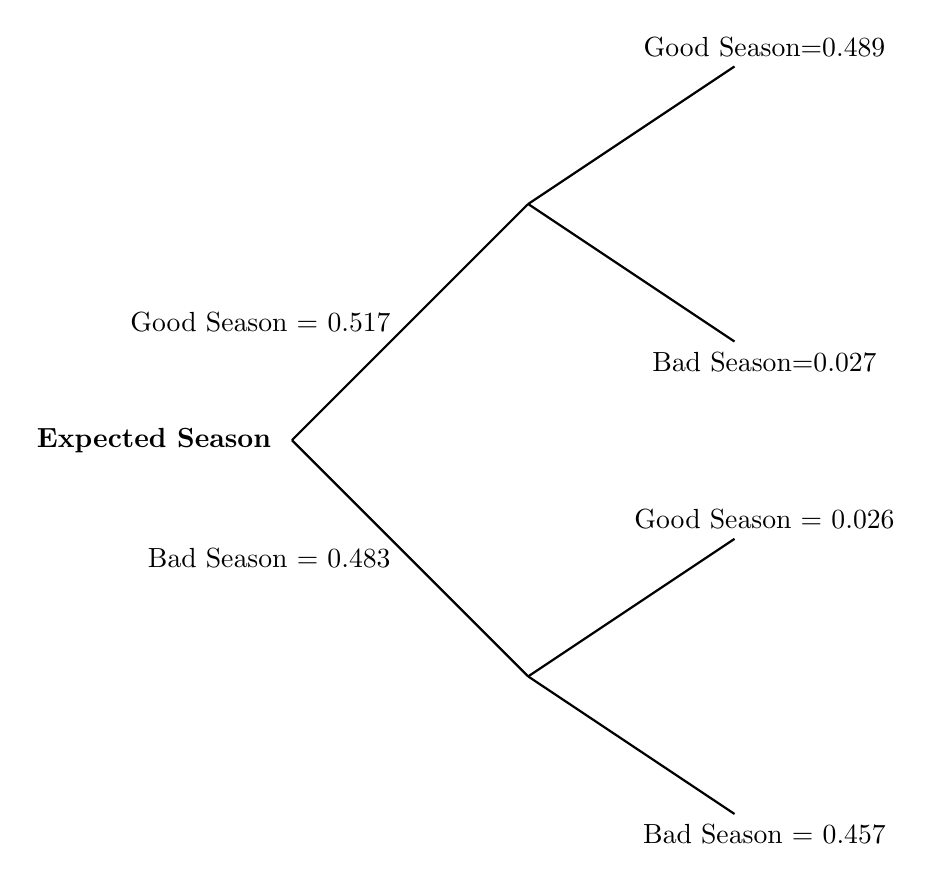
\begin{tikzpicture}[thick,
    level/.style={level distance=3cm},
    level 2/.style={sibling distance=6cm},
    level 3/.style={sibling distance=4cm}
]
\coordinate
child[grow=right, level distance=0pt] {
        child  {
            child {
                node {Bad Season = 0.457}
                edge from parent 
            }
            child {
                node {Good Season = 0.026}
                edge from parent
            }
            edge from parent
            node [left] {Bad Season = 0.483 \ }
        }
        child {
            child {
                node {Bad Season=0.027}
                edge from parent
            }
            child {
                node {Good Season=0.489}
                edge from parent  
            }
            edge from parent 
            node [left] {Good Season = 0.517 \ }
        }
        node [left] {\textbf{Expected Season\ \ }}
    };
\end{tikzpicture}
\end{figure}


\begin{figure}[htpb!]
\caption{Conception and Births: 40-45 Year-olds}
\hspace{8.0cm}\textbf{Realized Season} \vspace{4mm}\\
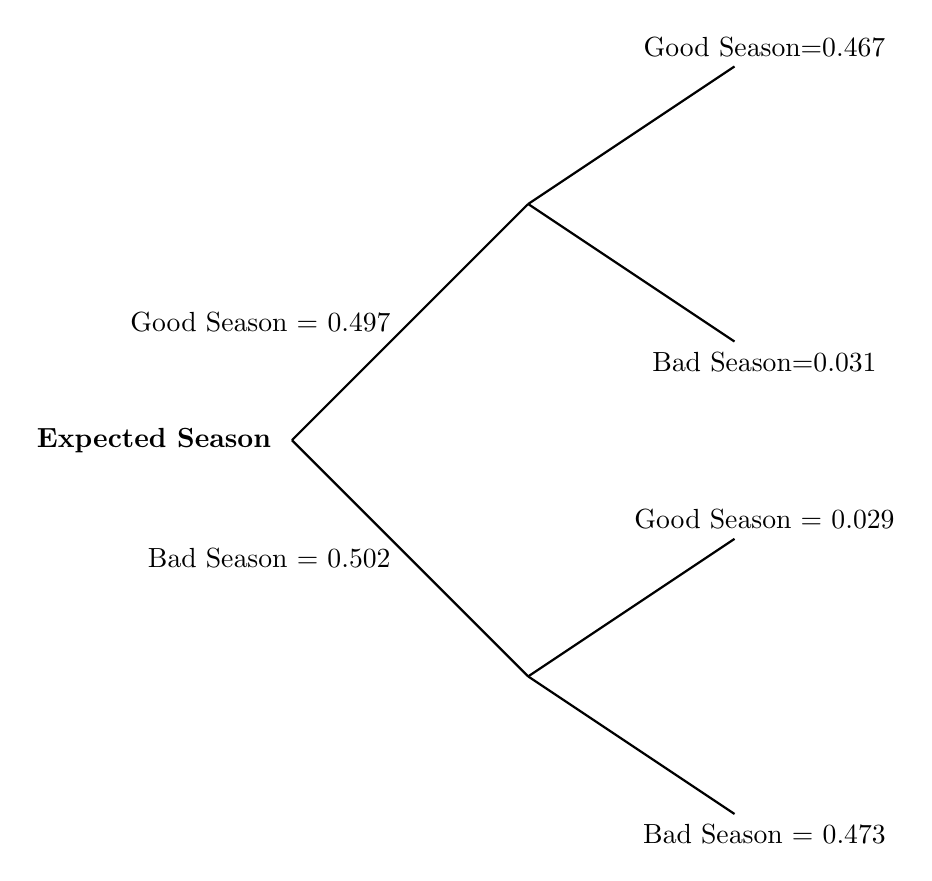
\begin{tikzpicture}[thick,
    level/.style={level distance=3cm},
    level 2/.style={sibling distance=6cm},
    level 3/.style={sibling distance=4cm}
]
\coordinate
child[grow=right, level distance=0pt] {
        child  {
            child {
                node {Bad Season = 0.473}
                edge from parent 
            }
            child {
                node {Good Season = 0.029}
                edge from parent
            }
            edge from parent
            node [left] {Bad Season = 0.502 \ }
        }
        child {
            child {
                node {Bad Season=0.031}
                edge from parent
            }
            child {
                node {Good Season=0.467}
                edge from parent  
            }
            edge from parent 
            node [left] {Good Season = 0.497 \ }
        }
        node [left] {\textbf{Expected Season\ \ }}
    };
\end{tikzpicture}
\end{figure}


\begin{figure}[htpb!]
\begin{center}
  \centering
  \caption{Good Season by State (Young)}
  \includegraphics[scale=0.34]{./../results/nvss/graphs/maps/young.png}
  \label{fig:mapYoung}
\end{center}
\end{figure}

\begin{figure}[htpb!]
\begin{center}
  \centering
  \caption{Good Season by State (Old)}
  \includegraphics[scale=0.34]{./../results/nvss/graphs/maps/old.png}
  \label{fig:mapOld}
\end{center}
\end{figure}

\begin{figure}[htpb!]
\begin{center}
  \centering
  \caption{Temperature and good Quarter: Young (Spain)}
  \includegraphics[scale=0.8]{./../results/spain/graphs/youngTempCold.eps}
  \label{fig:mapYoung}
\end{center}
\end{figure}
\clearpage

\begin{figure}[htpb!]
\begin{center}
  \centering
  \caption{Temperature and good Quarter: Old (Spain)}
  \includegraphics[scale=0.8]{./../results/spain/graphs/oldTempCold.eps}
  \label{fig:mapOld}
\end{center}
\end{figure}

\begin{figure}[htpb!]
\centering
\caption{Child quality: Birthweight (grams)}
\label{QBwt}
\includegraphics[scale=0.8]{../results/nvss/graphs/AllQuality_birthweight_.eps}
\end{figure}
\vspace{1cm}

\begin{figure}[htpb!]
\centering
\caption{Child quality: Birthweight (grams)}
\label{QApgar}
\includegraphics[scale=0.8]{../results/nvss/graphs/Quality_birthweight_.eps}
\end{figure}
\vspace{1cm}





\clearpage
\appendix
\section{Appendix Tables}
\input{./../results/nvss/regressions/NVSSBinaryFDeaths.tex}
\begin{table}[htbp]\centering
\def\sym#1{\ifmmode^{#1}\else\(^{#1}\)\fi}
\caption{Birth Quarter and Age (NVSS 2005-2013)}
\scalebox{0.8}{
\begin{tabular}{l*{4}{c}}
\toprule
                    &\multicolumn{1}{c}{(1)}   &\multicolumn{1}{c}{(2)}   &\multicolumn{1}{c}{(3)}   &\multicolumn{1}{c}{(4)}   \\
                    & Good Season   & Good Season   & Good Season   & Good Season   \\
\midrule
Aged 25-39          &       0.019***&       0.019***&       0.020***&       0.006   \\
                    &     [0.001]   &     [0.001]   &     [0.002]   &     [0.005]   \\
College Educ        &               &               &       0.010***&      -0.005   \\
                    &               &               &     [0.001]   &     [0.005]   \\
College$\times$ Aged 25-39&               &               &               &       0.015***\\
                    &               &               &               &     [0.005]   \\
Constant            &       0.497***&       0.497***&       0.488***&       0.501***\\
                    &     [0.001]   &     [0.001]   &     [0.002]   &     [0.005]   \\
\midrule
R-squared           &        0.00   &        0.00   &        0.00   &        0.00   \\
Observations        &     4871628   &     4871628   &     3613920   &     3613920   \\
Year FE&&Y&Y&Y\\ \bottomrule
\multicolumn{5}{p{12cm}}{\begin{footnotesize}Sample consists of all
first born children of US-born, white, non-hispanic mothers
\end{footnotesize}}\end{tabular}}\end{table}

\begin{landscape}
\input{./../results/bord2/regressions/NVSSQualityEducAll.tex}
\end{landscape}
\begin{landscape}
\begin{table}[htbp]\centering
\def\sym#1{\ifmmode^{#1}\else\(^{#1}\)\fi}
\caption{Birth Quarter and Age (NVSS 2005-2013)}
\scalebox{0.8}{
\begin{tabular}{l*{4}{c}}
\toprule
                    &\multicolumn{1}{c}{(1)}   &\multicolumn{1}{c}{(2)}   &\multicolumn{1}{c}{(3)}   &\multicolumn{1}{c}{(4)}   \\
                    & Good Season   & Good Season   & Good Season   & Good Season   \\
\midrule
Aged 25-39          &       0.019***&       0.019***&       0.020***&       0.006   \\
                    &     [0.001]   &     [0.001]   &     [0.002]   &     [0.005]   \\
College Educ        &               &               &       0.010***&      -0.005   \\
                    &               &               &     [0.001]   &     [0.005]   \\
College$\times$ Aged 25-39&               &               &               &       0.015***\\
                    &               &               &               &     [0.005]   \\
Constant            &       0.497***&       0.497***&       0.488***&       0.501***\\
                    &     [0.001]   &     [0.001]   &     [0.002]   &     [0.005]   \\
\midrule
R-squared           &        0.00   &        0.00   &        0.00   &        0.00   \\
Observations        &     4871628   &     4871628   &     3613920   &     3613920   \\
Year FE&&Y&Y&Y\\ \bottomrule
\multicolumn{5}{p{12cm}}{\begin{footnotesize}Sample consists of all
first born children of US-born, white, non-hispanic mothers
\end{footnotesize}}\end{tabular}}\end{table}

\end{landscape}
\begin{landscape}
\begin{table}[htbp]\centering
\def\sym#1{\ifmmode^{#1}\else\(^{#1}\)\fi}
\caption{Birth Quarter and Age (NVSS 2005-2013)}
\scalebox{0.8}{
\begin{tabular}{l*{4}{c}}
\toprule
                    &\multicolumn{1}{c}{(1)}   &\multicolumn{1}{c}{(2)}   &\multicolumn{1}{c}{(3)}   &\multicolumn{1}{c}{(4)}   \\
                    & Good Season   & Good Season   & Good Season   & Good Season   \\
\midrule
Aged 25-39          &       0.019***&       0.019***&       0.020***&       0.006   \\
                    &     [0.001]   &     [0.001]   &     [0.002]   &     [0.005]   \\
College Educ        &               &               &       0.010***&      -0.005   \\
                    &               &               &     [0.001]   &     [0.005]   \\
College$\times$ Aged 25-39&               &               &               &       0.015***\\
                    &               &               &               &     [0.005]   \\
Constant            &       0.497***&       0.497***&       0.488***&       0.501***\\
                    &     [0.001]   &     [0.001]   &     [0.002]   &     [0.005]   \\
\midrule
R-squared           &        0.00   &        0.00   &        0.00   &        0.00   \\
Observations        &     4871628   &     4871628   &     3613920   &     3613920   \\
Year FE&&Y&Y&Y\\ \bottomrule
\multicolumn{5}{p{12cm}}{\begin{footnotesize}Sample consists of all
first born children of US-born, white, non-hispanic mothers
\end{footnotesize}}\end{tabular}}\end{table}

\end{landscape}
\input{./../results/1970s/regressions/NVSSseasonMLogit.tex}
\input{./../results/1990s/regressions/NVSSseasonMLogit.tex}
\begin{landscape}
\input{./../results/1970s/regressions/QualityAllCombnoFE.tex}
\end{landscape}
\begin{landscape}
\input{./../results/1990s/regressions/QualityAllCombnoFE.tex}
\end{landscape}


\clearpage
\appendix
\section{Appendix Figures}
%\begin{figure}[htpb!] 
%\begin{center}
%  \centering  
%  \caption{Education and Conception Month}
%  \includegraphics[scale=0.7]{./../results/nvss/graphs/conceptionMonthDropout.eps}  
%  \label{fig:concepEduc} 
%\end{center}
%\floatfoot{\textsc{Notes to figure \ref{fig:concepEduc}}: Graph plots the proportion
%of conceptions by month for 25-39 year old women by education level.  Refer to figure
%\ref{bqFig:concepMonth} for additional notes.}
%\end{figure} 

\begin{figure}[htpb!]
\centering
\caption{Younger versus older women births (Spain)}
\label{bqFig:YoungvOldSpain}
  \centering
  \includegraphics[scale=0.82]{../results/spain/graphs/youngMonths.eps}
\floatfoot{\textsc{Notes to figure}: Each point and standard error comes from a regression
of birth month $x$ on a binary indicator of being young (25-39).
}
\end{figure}


\begin{figure}[htpb!]
\begin{center}
\caption{Temperature and Good Quarter (Spain)}
\label{fig:tempSpain}
\begin{subfigure}{.5\textwidth}
  \centering
  \includegraphics[scale=0.55]{./../results/spain/graphs/youngTempCold.eps}
  \caption{Young Mothers}
  \label{fig:tempSpainYoung}
\end{subfigure}%
\begin{subfigure}{.5\textwidth}
  \centering
  \includegraphics[scale=0.55]{./../results/spain/graphs/oldTempCold.eps}
  \caption{Old Mothers}
  \label{fig:tempSpainOld}
\end{subfigure}
\end{center}
\floatfoot{\textsc{Notes to figure}: See notes to figure 
\ref{fig:tempUSAYoung}. Monthly temperature data is 
collected from the Spanish State Meteorology Agency (AEMET).}
\end{figure}



\section{Data Appendix}
\label{bqScn:datApp}
\subsection{NVSS Birth Certificate Data}
A brief description of USA birth certificate data is provided in section 
\ref{bqSscn:USAdata} of the paper.  As discussed, the format of US birth
certificates has undergone two important revisions: the first in 1989
and the second in 2003.  The date of adoption of these revisions varies 
by state.  By 2013 41 states or territories had adopted the revised (2003)
format, while the reaminder still follow the 1989 format.\footnote{The full
birth certificate for each revision is reproduced as figures 1 and 2 in
\citet{MenackerMartin2005}.  Over time the adoption of the 2003 certificate 
was as follows: 2005: 12 (31\%), 2006: 19 (49\%), 2007: 22 (53\%), 2008: 27 
(65\%), 2009: 28 (66\%), 2010: 33 (76\%), 2011: 36 (83\%), 2012: 38 (86\%),
and 2013: 41 (90\%).  In each case the first number refers to the number
of states, while the parenthesis indicates the percent of births in revised
states.}

In all cases where variable coding differs between the revised and unrevised
certificates (principally education for mother and father), we use the revised
2003 coding of the variables.  The reason we do this is because after 2008,
variables which are exclusive to 1989 certificates are no longer reported.
Figure \ref{bqFig:educMissing} illustrates this pattern.  The dotted line 
represents the proportion of observations for maternal education which are
reported in the 1989 format, while the bars represent the proportion 
\emph{missing} in the 2003 format.  From 2005-2008, all missing 2003 revision
variables are recorded in the 1989 format.  However, from 2009 onwards only
the 2003 revision of education is reported, meaning that those states who
still use the 1989 standard certificate do not have publicly released education
data.  As expected, these are not missing at random, given that educational
attainment varies considerably by state (see table \ref{bqTab:missingEduc}).
In each case when these variables are used, we include full year and state
fixed effects.  
\begin{figure}[htpb!]
\caption{Missing Education Data by Time}
\label{bqFig:educMissing}
\includegraphics[scale=0.74]{../results/nvss/graphs/missingEduc.eps}
\end{figure}
\input{./../results/nvss/regressions/NVSSMissingScale.tex}


\end{spacing}
\end{document}







\begin{eqnarray}
\label{struc1}
\max_{\{s,a\}} u(w,b) &\text{s.t.}& w=f(age,educ,\mathbf{X},\varepsilon_w) \\ 
\label{struc2}
&& b=\mu(age,s,\mathbf{X},\varepsilon_b)                                  \\ 
\label{struc3}
&& s=\phi(age,educ,\varepsilon_s). 
\end{eqnarray}

Here $u(\cdot), f(\cdot), \mu(\cdot)$ and $\phi(\cdot)$ are functions and 
$\mathbf{\varepsilon}=(\varepsilon_w,\varepsilon_s,\varepsilon_b)$ are 
unobserved shocks.  To close the structural model we must attach functional
form to the four functions, and make distributional assumptions for $\varepsilon$.

Functional form for equations (\ref{struc2}) and (\ref{struc3}) can be quite simple, 
as it is precisely what we are estimating in equations (\ref{eqn:season}) and 
(\ref{eqn:quality}) respectively.  From our results we know very clearly that:
\[
\frac{\partial b}{\partial s^{good}}>0 \text{\ and \ }
\frac{\partial s^{good}}{\partial age}<0.
\]
It is also generally the case that:
\[
\frac{\partial w}{\partial age}>0.
\]
The wage equation in (\ref{struc1}) could be Mincerian, depending on $age$ and 
$age^2$, as well as education, and is calculated at the level of the state, 
(perhaps using data from CPS or similar to get wage).  Finally, we define $u(w,b)$ 
as a Cobb-Douglas
or CES function (or some other logical form), and assume that $\varepsilon$ is
drawn from a trivariate normal.  We can thus write down a log-likelihood function,
and use our birth data to maximise this function, estimating the parameters in
$f(\cdot), \mu(\cdot)$ and $\phi(\cdot)$, which allows us to quantify the
trade-off between ``having a child today'' versus ``having a child tomorrow'' 
with the relative (market and shadow) prices of labor, as measured by wages, and 
child quality, proxied by birthweights.
